\documentclass[../ECON-281-Notes.tex]{subfiles}
\begin{document}
\chapter{Monopoly}
\section{Characteristics of a Monopoly}
\begin{itemize}
    \item A single seller 
    \item High barriers to entry 
    \item Monopolist is the price maker or setter. 
\end{itemize}
Since the monopolist is the only seller his demand is the demand of the whole market which is negatively sloped. To sell more he has to lower the price.

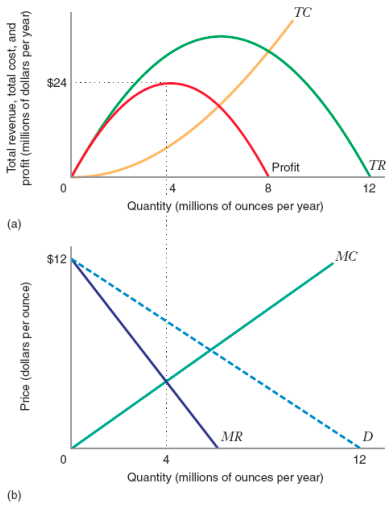
\includegraphics[width=\columnwidth]{assets/image-2021-12-11-12-25-07.png}

The \textbf{Marginal Cost} curve is the supply curve of the monopolist. However, the monopolist will only produce at a single point where $MC = MR$. 

\section{Objective}
The objective of any producer is to maximize profit. 
To maximize profit the monopolist must produce the quantity at which 
\begin{enumerate}
    \item \(MR = MC\)
    \item \(MC\) is rising.
\end{enumerate}


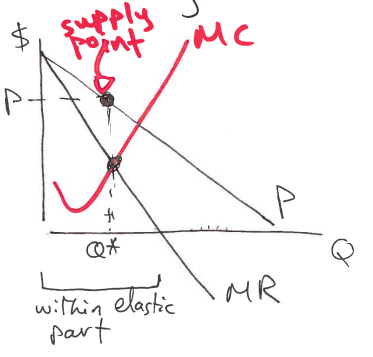
\includegraphics[width=\columnwidth]{assets/image_2021-11-23-12-09-44.png}
Monopolist must produce along the elastic part of his demand curve.
He will never produce along the inelastic part because MR is negative on that part.

\begin{Note}
    The monopolist has no supply curve. It has a supply point which is the point on his demand curve above the intersection of \(MR\) and \(MC\). 
\end{Note}

The \(Q^*\) is in between 0 and where \(MR > 0\), or at least on the elastic part on the demand curve. 

\section{Cases for Monopolistic Markets}
\begin{enumerate}
    \item Abnormal profit 
    \item Breakeven  
    \item Loss  
\end{enumerate}

The only difference between the three cases is the location of the ATC.
\newpage
\subsection{Abnormal profit}
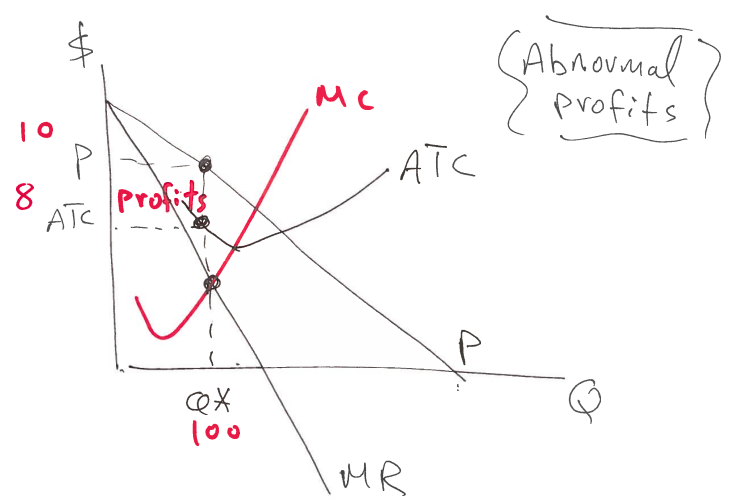
\includegraphics[width=\columnwidth]{assets/image_2021-11-23-12-10-51.png}

\subsection{Breakeven}
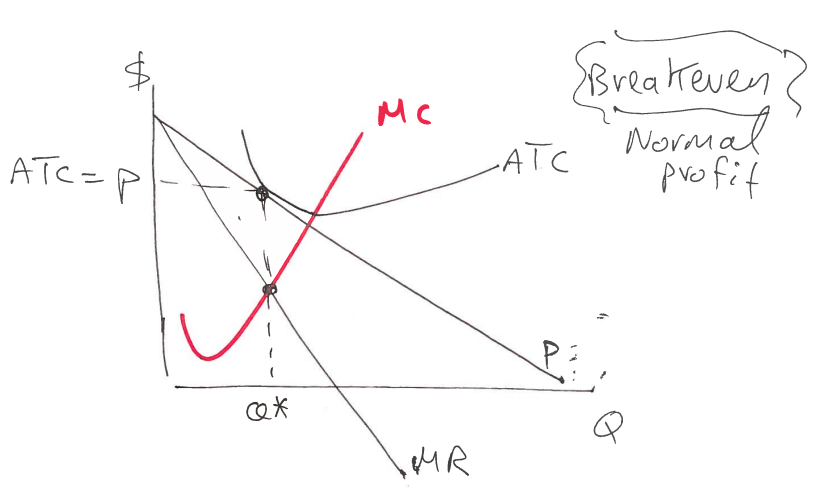
\includegraphics[width=\columnwidth]{assets/image_2021-11-23-12-11-32.png}

\subsection{Loss}
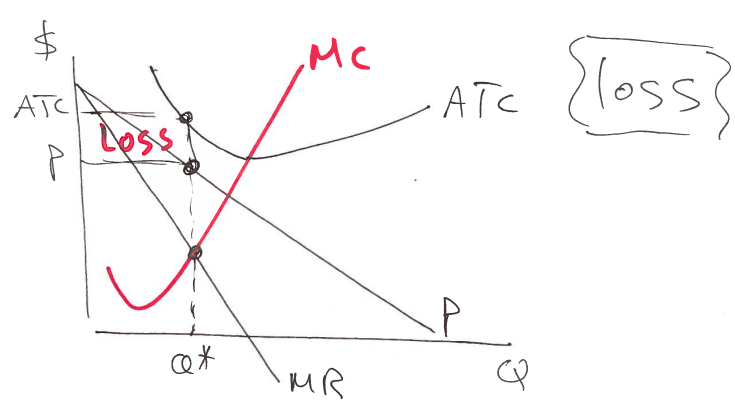
\includegraphics[width=\columnwidth]{assets/image_2021-11-23-12-11-51.png}


\section{Maximizing $TR$ vs Maximizing \(\Pi\) }

\begin{itemize}
    \item \textbf{Maximizing $\Pi$} is where \(MR = MC\)
    \item \textbf{Maximizing $TR$} is where \(MR = 0\)
\end{itemize}

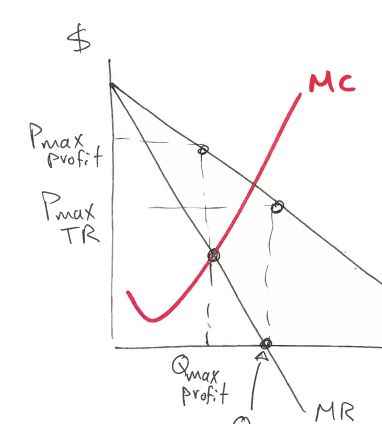
\includegraphics[width=\columnwidth]{assets/image-2021-12-11-12-42-48.png}

\begin{itemize}
    \item For quantity the \(Q_{TR} > Q_{\Pi}\)
    \item For price the \(P_{\Pi} > P_{TR}\)
\end{itemize}




\section{Monopoly vs Competitive Market}

Monopolist is bad because:
\begin{itemize}
    \item He produces a smaller \(Q\) and charges a higher \(P\) than perfect competition
    \item He generate a \(DWL\)
\end{itemize}

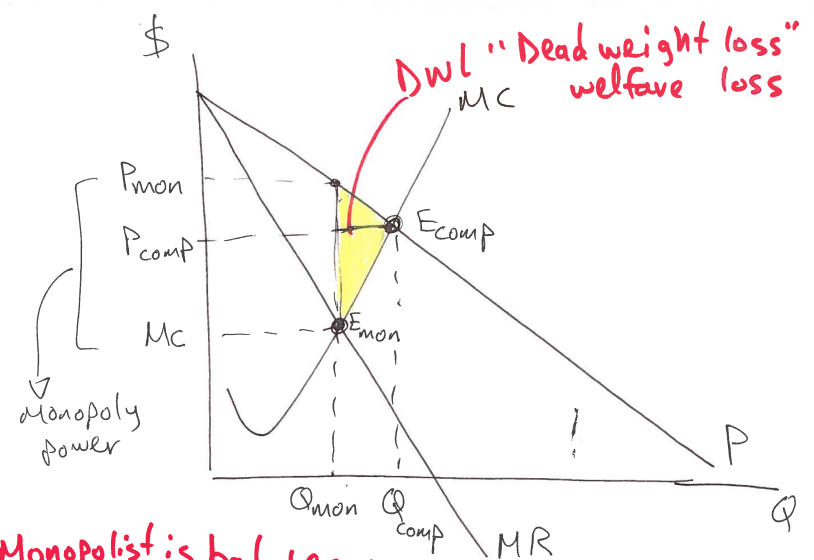
\includegraphics[width=\columnwidth]{assets/image_2021-11-23-12-13-29.png}

The difference between \(P\) and \(MC\) at the supply point determines the monopoly's power.
\newpage
\section{Monopoly Power}
Assume that: \[
    P = f(Q)
\]
\begin{align*}
    TR &= P \times Q\\
    MR &= \frac{\Delta TR}{\Delta Q} = \frac{\partial TR}{\partial Q}\\
    MR &= \frac{\Delta P}{\Delta Q} \times Q + P \\
    MR &= P \times \frac{\Delta P}{\Delta Q} \times \frac{Q}{P} + P \\
    MR &= P[1 + \frac{1}{\varepsilon_{Q.P}}]\\
    MR &= MC \\
    P + \frac{P}{\varepsilon_{Q.P}} &= MC\\
    P - MC &= \frac{-P}{\varepsilon_{Q.P}}\\
    \frac{P - MC}{P} &= \frac{-1}{\varepsilon_{Q.P}}
\end{align*}
The last term is the Learner's index of monopoly power.

The Learner's index of monopoly power measures the ability to change a price higher than $MC$.
The bigger the $\varepsilon_{Q.P}$ the smaller the monopoly power.

\newpage
\section{Comparative statics for monopolists}
Any shifts in the market demand or MC curves will cause a change int he monopolist equilibrium.

\subsection{Shifts in market demand}
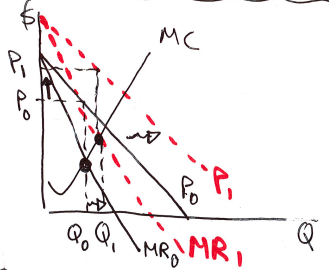
\includegraphics[width=\columnwidth]{assets/image_2021-11-29-22-52-41.png}
If market demand increases both the price and marginal revenue will shift right and the equilibrium price and quantity will rise.
The effect is the same in the opposite directions just everything flipped.

\subsection{Shifts in MC}
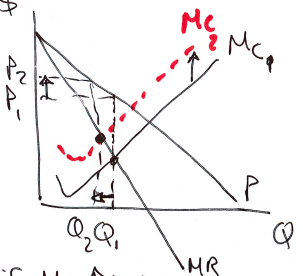
\includegraphics[width=\columnwidth]{assets/image_2021-11-29-22-54-08.png}
If the MC increase of shifts up the equilibrium quantity will decrease and the price will increase and since the monopolist produce in the \emph{elastic part} of his demand curve Total Revenue of the monopolist will decrease since the decrease in Quantity is greater than the increase in price.
The effect is the same in the opposite directions just everything flipped.



\section{Monopoly with multiple plants}
Consider a monopolist with two plants with marginal cost functions $MC_1$ and $MC_2$. 
How much would the monopolist produce overall and how should it divide that production between its two plants?

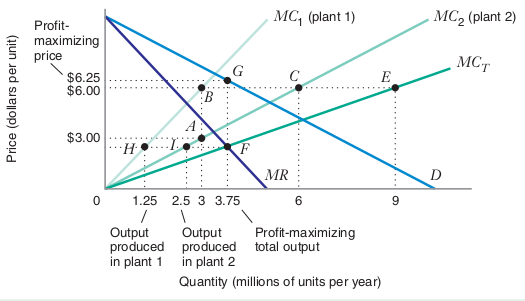
\includegraphics[width=\columnwidth]{assets/image_2021-11-29-23-01-08.png}

The total marginal cost is the horizontal sum of the individual plant's MC curves $Mc_1$ and $MC_2$.
Overall the monopolist produces $Q_T$ where $MC_T = MR$. 
To know how much each plant produces, we draw a horizontal line from the point of intersection of $MC_T$ and $MR$. Each plant will produce the quantity at which this drawn horizontal line cuts its $MC$ curve.

To get the horizontal sum, we must invert the MC equations by expressing $Q$ as a function of $MC$.

To determine $Q_{total}^{*}$ we need to get $MC_T$ and set it equal to $MR$. 
$MC_T$ is the horizontal summation of $MC$ of both plants.

\begin{Note}
  Be careful that we cannot add the given $MC$ equations as follows $MC_1+MC_2= 10 + 20Q_1 + 60 + 5Q_2$ here we are doing a vertical summation. To get the horizontal sum, we must invert the $MC$ equations by expressing $Q$ as a function of $MC$ as follows. 
\[ 
Q_1 = \frac{-1}{2} + \frac{1}{20} MC_1
\] 
\[ 
Q_2 = -12 + \frac{1}{5} MC_2 
\] 
The variable $Q$ is the responding variable, not $MC$.
\end{Note}

The sum of the two $Q$s will give you $Q_T$, in this case $Q_T = -12.5 + 0.25 MC_T \to MC_T = 50 + 4 Q_T$ 

To get $Q_T^*$ set $MR = MC_T$ solving the equation will give you the equilibrium quantity and from there you can get the price by substituting it into the market demand equation.

To determine allocation of production between the two plants, we calculate $MC_T$ at the point of intersection of $MC_T$ and $MR$. This value can be obtained by substituting $Q_T^* = 7$ into $MR$ or $MC_T$. This value will be $78\$ $.
By substituting  
\begin{Definition}
  {Cartel} 
  Group of producers that collusively determine $P$ and $Q$ in the market.

  The way this works is similar to the monopolist multi-plant production as shown in the previous section.
\end{Definition}

\end{document}
